\chapter{Pruebas de concepto}

\section{Primeros prototipos}
Antes de analizar las capacidades de las librerías sin marcadores se realizaron algunos prototipos en los que se ponía a prueba las funcionalidades con marcadores. De esta manera nos permitió conocer las diferencias entre ambos tipos de aplicaciones. Una vez conocidas estas diferencias se desarrollaron prototipos en los que se pone a prueba las funcionalidades de la realidad aumentada sin marcadores. Seguimos este orden de desarrollo para ir avanzando por las diferentes etapas por las que ha pasado este campo en todo su proceso evolutivo. Estos prototipos se describirán a lo largo de las siguientes secciones.

\subsection{Pruebas con ARToolKit}
En nuestros primeros pasos en el mundo de la realidad aumentada exploramos algunas librerías como ARToolKit, con el fin de familiarizarnos con el desarrollo de este tipo de aplicaciones.\\

ARToolKit es una de las librerías de desarrollo pioneras en el ámbito que investigamos, disponible desde el año 2004 para descargar de manera gratuita y que cuenta con más de 160.000 descargas desde entonces. Se distribuyó para diversas plataformas como SGI IRIX (que dejó de utilizarse en 2006), Linux, MacOS y Windows y fue desarrollada originalmente por el Dr. Hirokazu Kato para posteriormente pasar a manos del Human Interface Technology Laboratory en la Universidad de Washington y ARToolworks.Inc en Seattle.\\

Muchas librerías posteriores se han basado en el código de ésta para ampliar sus funcionalidades, dando lugar a algunas como ARTag (que promete mayor fiabilidad a la hora de procesar imágenes por su mejor manejo de la luz), FLARToolKit (consistente en un \textit{port} en ActionScript 3), ARDesktop (que facilita la creación de interfaces) o\textit{ Studierstube Tracker} (que mejora sus características, pero deja de ser de código abierto).\\
Además de todas las derivaciones de ARToolKit, también podemos encontrar software no orientado a programadores como ATOMIC Authoring Tool, que permitía a cualquier usuario el desarrollo de una aplicación de realidad aumentada de manera sencilla y con una interfaz intuitiva. Esta herramienta acabó cayendo en desuso a principios de la década de 2010 debido a que ya existían librerías mejores que ARToolKit y mejores alternativas en lo que a SDK se refiere.\\

Al ser ARToolKit una de las primeras herramientas para el desarrollo de realidad aumentada, no contemplaba un uso de esta sin marcadores. Una de las mayores dificultades a las que se enfrentó fue el seguimiento del “ojo” del usuario, es decir, el foco de la cámara del dispositivo. Para saber desde qué perspectiva debía dibujar los elementos virtuales la aplicación necesitaba saber a dónde está mirando el usuario en el mundo real. La librería solventa este problema utilizando algoritmos de visión que calculan la localización y orientación de la cámara basándose en marcadores físicos en tiempo real.
Los marcadores que es capaz de identificar consisten en la mayoría de los casos en un cuadrado negro bien contrastado con un fondo e interior blancos. Además, cada marcador, para diferenciarse del resto incluye pequeñas variaciones como otras figuras geométricas dentro del cuadrado.\\

Para nuestros experimentos con ARToolKit, en lugar de utilizar la librería original, utilizamos una adaptación de la misma para ser utilizada en Unity3D, que puede encontrarse actualmente en \url{https://github.com/artoolkit/arunity}. Esta extensión nos permite el acceso a componentes como \textit{ARController} y \textit{ARMarker} dentro del editor.\\

Para el desarrollo de este “HolaMundo” con ARToolKit en Unity hemos seguido los siguientes pasos: creamos un \textit{GameObject}\footnote{Objeto de Unity3D}  que servirá como “raíz” de la escena y otro que actuará como gestor del sistema de realidad aumentada. Al gestor le incluimos el componente \textit{ARController}, que está encargado de las opciones de vídeo y del seguimiento de los marcadores. Dentro de éste modificamos la capa a la que debe prestar atención. \\

Por otra parte, el objeto raíz de la escena incluye la luz direccional y la cámara, y además le añadimos el \textit{script} \textit{AROrigin}, que permite situar espacialmente la escena. La cámara, además de su \textit{script} de cámara por defecto, debe recibir el componente \textit{ARCamera} para poder detectar los marcadores.\\

Ahora hay que crear un objeto que llevará la información del marcador y le añadimos el componente \textit{ARMarker}, que lleva la etiqueta del marcador que hace de identificador único. Este componente tiene dos tipos de patrones (figura~\ref{TipoARTK}) para identificar por defecto: \textit{hiro} y \textit{kanji}. En este caso utilizaremos el patrón \textit{hiro}.\\

\begin{figure}[H]
    \centering
    \includegraphics[width=0.7\linewidth]{Images/Patron_ARTK.png}
    \caption{Tipos de patrón ARToolkit\footnotemarker}
    \label{TipoARTK}
\end{figure}

Añadimos a la raíz de la escena un objeto que será contenedor del objeto 3D que queremos que aparezca cuando enfocamos al marcador y que lleva el script \textit{ARTrackedObject} y dentro del campo \textit{Marker Tag} introducimos el identificador del marcador asociado al objeto.\\

\subsubsection{Conclusiones:}
Si bien esta librería fue útil en su día para sentar las bases del desarrollo de programas en realidad aumentada, hoy en día no se encuentra  documentación actualizada  y la página web que le daba soporte ha desaparecido~\cite{artoolkit_web}. Además, sus funcionalidades son muy limitadas y su rendimiento es muy inferior al que presentan otras alternativas más actuales como Vuforia, que permite también el uso de marcadores.\\

\subsection{Harry Potter}
\textbf{Se pueden ver los resultados en el vídeo \url{https://vimeo.com/331236805}.}\\

Después de descartar ARToolkit, nos decantamos por hacer las pruebas con Vuforia, que tiene soporte tanto para realidad aumentada con marcadores como sin ellos. Además, la documentación es reciente y ofrece una serie de posibilidades que nos interesaba aprovechar, como por ejemplo su integración con Unity3D.\\

Para implementar los prototipos pensamos en aplicaciones que fueran rápidas de codificar, pero que pudieran aportar algo interesante a los ojos de los usuarios. Tras un tiempo de debate encontramos curiosa la idea de que “escaneando” con el móvil un cartel o las viñetas de un cómic se pudiese obtener información no presente a simple vista en el mundo real, aportándole una capa más de profundidad y dinamismo a la experiencia del observador. A continuación comentamos el proceso de desarrollo.\\

Suscribiéndonos a la web de Vuforia se nos da la posibilidad de crear una base de datos con imágenes que nosotros mismos tomemos o escojamos para la aplicación. Este servicio de Vuforia ofrece un número limitado de bases de datos que podemos crear, pero es posible expandirlo y encontrar otras funcionalidades con los planes Basic o Pro. En nuestro caso no lo consideramos necesario y procedimos a buscar una imagen que nos sirviese como marcador. En esta primera aproximación nos basamos en los periódicos mágicos que aparecen en la saga de películas de Harry Potter y encontramos la página del periódico en la que aparece el prisionero de Azkaban (la cárcel de este universo literario). Al subir al servidor de Vuforia la imagen, la web nos muestra una estimación de cuánto de reconocible es el marcador basándose en el contraste que existe entre la saturación de las distintas partes en las que divide la foto (figura \ref{VufEst}). Se nos señalan los principales puntos de la foto que usará la librería para identificar el marcador. Cuantos más haya y más repartidos estén mejor será su calidad. De esta forma se puede decidir como desarrollador si utilizar cierta imagen como marcador o buscar otra con unas características mejores y que haga la experiencia más cómoda de cara al usuario.\\

\begin{figure}[H]
    \centering
    \includegraphics[width=0.9\linewidth]{Images/vuforiaMarks.jpg}
    \caption{Estimación de Vuforia}
    \label{VufEst}
\end{figure}

Como explicábamos, nosotros utilizamos la imagen que incluimos en la figura \ref{Azkaban}, recortando el cuadrado en el que aparece la foto del preso que es la que utilizaremos como marcador. A continuación tuvimos que buscar el fragmento animado del periódico que aparece en la película, que no nos llevó mucho tiempo puesto que debido a la popularidad de la saga estaba disponible en varias páginas web. Después ajustamos con un editor el tamaño del vídeo para que coincidiera con las dimensiones de la foto, como podemos observar en la imagen de la figura~\ref{Azkaban}.\\

\begin{figure}[H]
    \centering
    \includegraphics[width=0.6\linewidth]{Images/DailyProphetAzkaban.jpg}
    \caption{Aplicación del periódico de Harry Potter}
    \label{Azkaban}
\end{figure}

Ahora viene el momento de utilizar Unity. Desde el editor, y con el paquete de Vuforia instalado procedimos a importar la base de datos que nos da Vuforia con la ilustración convertida en marcador. Realizar un uso básico y a modo de prueba de esta librería para el desarrollo de un ejemplo en RA es bastante sencillo ya que puede hacerse incluso sin escribir una sola línea de código.\\

Necesitamos en la escena un objeto que sea del tipo \textit{AR Camera}, que se encargará de renderizar la escena y detectar los marcadores. Usando este objeto podemos prescindir de la cámara tradicional. A continuación introdujimos el objeto \textit{Image Target}, también dentro del paquete de Vuforia y lo configuramos para que el componente \textit{Image Target Behaviour} utilice la base de datos que tenemos y la imagen que le corresponde. Como hijo del \textit{Image Target} incluimos el objeto virtual que queremos que aparezca al encontrar el marcador. En este caso, un objeto del tipo \textit{Quad} (es decir, un rectángulo vacío) nos servirá. Ajustamos el ancho y el alto al tamaño del padre y le añadimos el componente \textit{Video Player} para que reproduzca el vídeo. Con esto sólo necesitamos compilar la aplicación y pasar el archivo a un móvil que lo soporte para probar la aplicación.\\


\subsection{DragonBall}

\textbf{Se pueden ver los resultados en el vídeo: \url{https://vimeo.com/331236593}.}\\

La siguiente aplicación que desarrollamos está impulsada por la idea de leer un cómic en realidad aumentada. Utilizamos una página del manga de Dragon Ball para este ejemplo y le aplicamos el mismo procedimiento que al programa anterior, aunque con un par de excepciones, puesto que la cámara ahora en lugar de llevar el \textit{tracking} de un solo marcador, lleva uno por cada viñeta. De esta forma se reproducen los cuatro vídeos a la vez.\\

En primer lugar, escogimos una página con unas viñetas nítidas para que los marcadores tuvieran suficientes características distintivas como para que Vuforia las reconociese con facilidad. Una vez seleccionada (figura~\ref{DBZ}) continuamos con el proceso de subida al servidor de Vuforia para obtener la base de datos. La parte difícil vino a continuación, pues tuvimos que encontrar el capítulo de la serie animada en el que sucedieran los hechos de esa página del cómic, para después recortar los fragmentos correspondientes a cada viñeta y ajustar el breve vídeo de cada una al tamaño justo de la misma. Una vez teníamos todos los recursos ya sólo había que introducirlos en el editor de Unity, creando esta vez cuatro \textit{Target Images} (uno para cada viñeta) y un \textit{Quad} con el vídeo propio para cada uno.\\

El resultado es muy vistoso y puede llegar a convertirse en una forma de ampliar la inmersión o mejorar la experiencia de los lectores habituales.

\begin{figure}[H]
    \centering
    \includegraphics[width=0.7\linewidth]{Images/mangaKrillin.jpg}
    \caption{Página del cómic con RA}
    \label{DBZ}
\end{figure}

Cabe destacar que actualmente la tecnología está limitada en este ámbito, ya que pese a que muchos dispositivos como tabletas o móviles soportan la realidad aumentada con marcadores es de cierta manera incómodo tener que estar enfocando con la cámara al lugar en cuestión para obtener la información o la experiencia adicional y resulta cansado después de unos cuantos usos.


\subsection{Juego de cartas Yu-gi-oh}

\textbf{Se pueden ver los resultados en el vídeo \url{https://vimeo.com/331237916}.}\\

Llegados a este punto, queríamos comprobar cómo sería el desarrollo de un juego que utiliza realidad aumentada con marcadores. Nos basamos para ello en el juego de cartas de Yu-Gi-Oh, que tiene su origen en un cómic japonés del mismo nombre y que alcanzó gran popularidad en la década de los 2000 en todo el mundo. El juego es de temática similar al de las cartas Magic, en el que cada carta representa un monstruo, cada uno con sus propios atributos, valores de ataque y defensa y otras características, que se enfrentan contra los monstruos del oponente siguiendo un sistema de reglas y turnos bastante complejo. Además de las cartas de monstruo existen otras que modifican los valores de las mismas o tienen otros efectos en la partida. Para facilitar el desarrollo, simplificamos todas estas condiciones y nos centramos en algunos aspectos esenciales: la partida se va sucediendo por turnos, las criaturas pertenecen a uno u otro jugador según su posición en la mesa y dentro de un turno el jugador puede decidir si el monstruo que está bajo su control ataca o defiende.\\

Lo verdaderamente interesante de este juego es que en la saga de cómic (y posterior serie animada de televisión) los jugadores juegan sobre un tablero electrónico sobre el que colocan las cartas y aparece una representación holográfica de las criaturas de las mismas. Esta tecnología de ciencia ficción se escapa un poco de nuestro alcance y presupuesto, pero sí que podemos intentar una recreación más simple con nuestros conocimientos de realidad aumentada y ver a los monstruos por medio de la pantalla de nuestros dispositivos móviles, como ya hicieron anteriormente juegos como Invizimals en 2009 o Pokémon Go en 2016.\\

Para desarrollar esta aplicación volvimos a utilizar el motor Unity con Vuforia. Utilizamos dos cartas del juego como marcadores para que durante el uso del programa proyectaran los modelos 3D de los monstruos correspondientes. Para los modelos buscamos algunas de las criaturas más conocidas de la franquicia y así evitamos tener que realizar nosotros a mano el proceso de modelado y generación de texturas. Encontramos en la página ``The model resource''\footnote{ \url{https://www.models-resource.com}} los personajes que buscábamos (Kuriboh y Jinzo) y seleccionamos las cartas con sus imágenes para crear la base de datos que contendría los marcadores.\\

Aunque los modelos encontrados eran correctos, carecían de animaciones, lo que limitaba la calidad del resultado. Sin embargo, en sus respectivos archivos sí pudimos encontrar un \textit{rigging}\footnote{ Proceso de crear un sistema de controles digitales y agregárselos a un modelo 3D para que así pueda ser animado fácilmente y eficientemente} básico (esqueleto animable).
Por esto, nos aventuramos a utilizar Blender, un programa de modelado, iluminación, renderizado y animación entre otras muchas características con el que estamos familiarizados por su uso en varios proyectos durante el grado y que además es software libre. Realizamos animaciones de estado de reposo, ataque, defensa, movimiento y de recibir daño para ambas criaturas, además de las transiciones entre estos estados para evitar saltos poco realistas e incómodos en la simulación.\\

Una vez guardadas todas las animaciones, el propio archivo de Blender puede ser directamente importado a Unity para utilizar todos los objetos y texturas que se encuentran en él. Esto nos facilitó mucho el trabajo al no tener que convertir los modelos a otro formato con la posible pérdida de información en los modelos o las animaciones. Una vez dentro del editor creamos los objetos que servirían como marcadores y les asignamos a cada uno su imagen correspondiente de la base de datos proporcionada por Vuforia. Como objeto hijo de cada marcador, le asignamos la figura correspondiente y creamos un \textit{prefab} con todo ello, ya que de querer ampliar el juego con más cartas cada una debería hacer referencia a un monstruo distinto.\\

Llegó la hora de ponernos a codificar. Establecimos un objeto vacío que sirviese de \textit{Game Manager} y llevase la lógica del juego, es decir, el transcurso de los turnos y las elecciones del jugador. Para empezar a jugar se sitúan las cartas sobre la mesa, una frente a la otra. Basándose en la orientación inicial de los marcadores cuando son detectados por la cámara, el juego asigna cada criatura al jugador al que le pertenece. Una vez pasada esta fase de reparto, le toca el turno al primer participante, que debe seleccionar uno de los monstruos en su control. Una vez hecho esto, aparecen tres botones en la pantalla: dos de ellos son para decidir si la criatura debe atacar o defender y el tercero cancela la selección y vuelve a la fase en la que se pide que escojas un monstruo. Si escoges atacar, el siguiente paso será buscar al objetivo del ataque, para lo que se pedirá seleccionar uno de los enemigos. Acto seguido, tu criatura se dirigirá a la del rival, la atacará haciéndole daño (que repercutirá en sus puntos de vida) y volverá a su carta de origen para pasar al turno del contrincante. Si por el contrario se elige la opción de defensa, el monstruo adoptará una postura defensiva que le permitirá cubrirse de los ataques enemigos y al acabar terminará el turno actual. A continuación será el turno del rival, que tendrá las mismas posibilidades, aunque en este caso jugaremos contra la máquina y sus acciones serán reducidas.\\

Para gestionar todo el grafo de animaciones necesitamos un objeto \textit{Animator Controller} que lleve las condiciones para pasar de un estado al siguiente y volver para cada uno de los modelos. Todos estos cambios se recogen a nivel de código una vez pulsamos los botones de selección de acción.\\

\begin{figure}[H]
    \centering
    \includegraphics[width=\linewidth]{Images/YuGiOh.jpg}
    \caption{Visualización del juego de cartas}
    \label{YuGi}
\end{figure}

Con estas pequeñas muestras habríamos terminado nuestra incursión en la realidad aumentada con marcadores y estaríamos preparados para el siguiente paso, en el que prescindiríamos de ellos.

\subsection{JengAR}
\textbf{Se pueden ver los resultados en el vídeo \url{https://youtu.be/TzndzVwH3rI}.}\\
Este prototipo fue creado para probar la realidad aumentada sin marcadores y la interacción con objetos virtuales, añadiendo la posibilidad de cambiar el punto de ancla de algunos objetos sobre la marcha y moviendo el resto de objetos de forma natural usando físicas. 
Decidimos desarrollar un prototipo rápido donde se instancia una pila de bloques en un plano. Si nos acercamos un bloque y mantenemos pulsado la pantalla, el bloque se ancla a nuestro movimiento, por lo que hay que realizar movimientos suaves y cuidadosos, para no tirar la torre.\\

Cuando se pulsa la pantalla se calcula el punto que se encuentra en la mitad de la pantalla y se lanza un \textit{raycast}\footnote{Rayo que se lanza desde un punto origen hasta un punto final para comprobar si existe algún elemento en el camino}, si éste detecta un bloque, se marca como seleccionado, se fija la distancia entre su posición y la nuestra, y empieza a moverse junto a nosotros, manteniendo la distancia inicial.\\

En la figura \ref{JenAR} se pueden observar algunas capturas de la aplicación.
\begin{figure}[H]
    \centering
    \includegraphics[width=\linewidth]{Images/Jenga.jpg}
    \caption{Visualización del JengAR}
    \label{JenAR}
\end{figure}

\section{Pruebas de concepto}
Una vez desarrollados los prototipos y haber estudiado las posibilidades de la realidad aumentada, propusimos crear pruebas de concepto más complejas que tuvieran utilidad en el día a día. Decidimos desarrollar tres aplicaciones:
\begin{itemize}
    \item Aplicación instructiva (AmueblAR), que permite visualizar el proceso de montaje de un mueble en realidad aumentada, sin necesidad de observar las instrucciones en un papel plano.
    \item Aplicación inmersiva (Visualizer 3D), útil para observar y manipular modelos 3D en tiempo real.
    \item Un videojuego multijugador online (BombARdero+), en el que se puede jugar desde distintos dispositivos a la vez.
\end{itemize}

\subsection{Instrucciones de montaje de muebles en AR - AmueblAR}
\textbf{Se pueden ver los resultados en el vídeo \url{https://youtu.be/o-N_Jpdt9Do}.}\\
En nuestra investigación hemos visto que una utilidad popular en el campo de la realidad aumentada sin marcadores son las aplicaciones de decoración de interiores (sección~\ref{ecommerce}). Ikea, por ejemplo, ha lanzado Ikea Place, una aplicación de realidad aumentada para dispositivos móviles que permite visualizar cualquier habitación de tu casa con muebles virtuales. De esta manera podemos decidir si encajan con nuestro salón y si las medidas son las adecuadas para después comprar el mueble en la tienda física.\\

Sabemos que comprar sofás o estanterías por piezas es en ocasiones más barato y facilita enormemente el transporte, sin embargo la parte en la que muchos compradores experimentan problemas es a la hora de montarlos. Muchos son incapaces de ver en el plano de las instrucciones en qué lugar va cada tornillo o de qué forma se unen las patas. Por eso, la aplicación que nosotros hemos propuesto consiste en un pequeño manual de instrucciones en realidad aumentada sin marcadores. De esta manera se puede ver en todo momento el modelo 3D del mueble, rotarlo y además desplazarte alrededor de él para apreciar en detalle cada uno de los pasos en el proceso de montaje.\\

El funcionamiento es muy sencillo: para empezar escaneamos el plano para que el programa cree una superficie donde colocar el mueble. A continuación tocamos la pantalla en el lugar en el que queremos colocarlo. Ahora podemos rotar el mueble hacia izquierda y derecha para dejarlo en una posición en la que nos resulte cómodo acercarnos y alejarnos mientras vemos los pasos de montaje. Finalmente, al pulsar el botón de aceptar entramos en la fase de construcción. En ella tenemos un botón a cada lado de la pantalla: el de la izquierda retrocede al paso anterior y el de la derecha avanza al paso siguiente. Mientras se suceden las animaciones que van explicando cómo armar progresivamente el mueble el usuario puede moverse libremente con su dispositivo para apreciar los detalles e incluso retroceder si no ha entendido bien el paso a seguir.\\

Para el desarrollo hemos utilizado la librería ARCore en Unity, que permite el despliegue de realidad aumentada sin marcadores. Utilizando la tecnología que nos vienen dada por la librería buscamos una serie de puntos en el suelo que nos permitirán crear un plano virtual. Una vez generada esta superficie el plano se representa gráficamente en pantalla con la unión de los puntos. A continuación dividimos la aplicación en tres estados: despliegue, rotación y montaje.\\ 

Empezamos en la fase de despliegue, en la que el programa está continuamente esperando la interacción del usuario. Cuando se toca la pantalla, se comprueba si ha habido colisión con el plano virtual, y de ser así se instancia el mueble en el lugar en el que hemos tocado. Si este proceso se ha llevado a cabo con éxito, pasamos a la fase de rotación. Aquí aparecen dos botones azules a los lados de la pantalla y uno verde en la parte inferior. Los botones laterales llevan una referencia al mueble para que al ser pulsados lo roten en una u otra dirección. El botón inferior por otra parte nos sirve para comunicarle a la aplicación que estamos conformes con la posición actual del objeto y que puede pasar a la siguiente fase.\\ 

Finalmente nos encontramos con dos nuevos botones a los laterales, que como hemos explicado anteriormente se encargan de adelantar y retroceder los pasos de montaje. El sofá tiene un componente \textit{Animator Controller} que lleva el árbol de estados. Este árbol consta de 10 estados fijos, en los que se queda el mueble una vez ha terminado su animación correspondiente y 18 estados móviles o animaciones, que se reproducen cuando se pulsan los botones de avanzar o retroceder. Para ello, existe una variable que controla el avance y otra que hace lo propio con el retroceso, que se anulan una vez se entra en un estado estático y se activan al pulsar el botón que corresponde, pasando así a la animación del paso siguiente o anterior.\\

Cabe destacar el proceso de creación del mueble en sí mismo, que en el caso del ejemplo se trata del sofá \textit{Kivik}. Como no era posible encontrar un modelo dividido en piezas y fácilmente animable se realizó un modelo desde cero con la ayuda de la documentación que encontramos en la web de Ikea. El mueble consta de las siguientes piezas: el asiento del sofá, el respaldo del sofá, el asiento de la \textit{cheslong} \footnote{ Tipo de sofá que posee una prolongación lo suficientemente larga en forma de L como para soportar las piernas humanas.} y su respaldo, los dos brazos, dos escuadras, una pletina, ocho patas, dieciocho tornillos con sus correspondientes tuercas y arandelas, cinco cojines cuadrados y un cojín alargado para la \textit{cheslong}. Excluyendo los tornillos, que los encontramos en una página de recursos gratuitos~\cite{tornillos}, todos los demás fueron creados por nosotros en Blender, herramienta de la que ya hemos hablado anteriormente. Una vez terminadas las piezas del sofá, las texturizamos con colores azules y aspecto de sofá, y por otro lado las piezas como los tornillos o las escuadras una textura metálica.\\

Pensamos que podríamos empezar a animar cada parte por separado dentro de un objeto conjunto del que fueran hijas todas las piezas, pero para que Unity pueda interpretar cada acción como propia de un objeto mayor a las partes es necesario hacer un \textit{rigging} que abarque todas piezas del sofá. Una vez construido el esqueleto se le asigna a cada hueso el objeto que se va a encargar de mover. Este proceso ocasionó algunos problemas, al tratarse de un objeto compuesto ciertos huesos acababan emparentándose automáticamente con partes del sofá que nos les correspondían. La única solución fue establecer manualmente los pesos (es decir, la influencia que tiene cada hueso sobre una parte concreta) sobre los diferentes conjuntos de vértices hasta que conseguimos el resultado que esperábamos.\\

En lo referente a las animaciones nos fue muy útil el vídeo que tiene publicado la cuenta de Ikea España en la plataforma Youtube~\cite{IkeaYT} en el que se explica el procedimiento que se sigue para construir el sofá. Habiéndolo analizado dividimos el montaje en 9 pasos diferenciados y los animamos también en Blender, haciendo desaparecer las partes que no se están utilizando en ese momento para que sea más claro y fácil verlo.\\

Al contrario que en los ejemplos con marcadores en los que pudimos exportar directamente el archivo de Blender para su uso en Unity, aquí nos dio problemas ya que el editor dejó de reconocer los \textit{clips} de vídeo de algunas animaciones. Solventamos este problema exportando el objeto desde el programa de modelado en formato ``fbx'', pero nos surgió otro nuevo inconveniente, todas las partes del sofá habían perdido sus texturas. Ya desde Unity creamos los materiales por separado y se los asignamos a cada pieza.
Fue un proceso bastante agotador, pero consideramos que el resultado es satisfactorio y útil, además ofrece nuevas posibilidades en un campo que no deja de crecer.\\

\begin{figure}[H]
    \centering
    \includegraphics[width=\linewidth]{Images/amueblar.jpg}
    \caption{Capturas de la aplicación AmueblAR}
    \label{mueblAR}
\end{figure}

\subsection{Visualizador de objetos en AR con gafas Aryzon - Visualizer 3D}
En la fase de investigación, pensamos que una de las limitaciones de la realidad aumentada en dispositivos móviles es el hecho de tener que sujetar el móvil con las manos, por lo que el control y la experiencia de usuario se ve condicionada negativamente. Una vez identificamos este problema decidimos buscar un \textit{headset low cost} de realidad aumentada, encontrando las gafas de Aryzon \cite{Aryzon}. Se trataba del producto perfecto para iniciarnos en el desarrollo de RA con \textit{headset}.\\

Decidimos desarrollar una aplicación en la que se pudiera ver objetos y/o modelos 3D y poder caminar alrededor de ellos. Para añadirle más funcionalidad, usamos un mando de \textit{Xbox One} que nos permitirá mover, rotar y escalar el modelo a nuestro gusto, con el objetivo de poder manipular la aplicación sin necesidad de tocar el móvil, ya que éste estará colocado en las gafas.\\

Para el desarrollo de la aplicación usamos el SDK de Aryzon, ya que nos facilita la vista estereoscópica para simular los ojos y ARCore para la tecnología de realidad aumentada.\\

Se decidió usar la detección de planos de ARCore, ya que queríamos usar la realidad aumentada sin marcadores y movernos alrededor del modelo, y como hemos visto en las pruebas, la estabilidad de los puntos de anclaje de ARCore es muy buena.\\

Para el desarrollo de esta prueba de concepto, necesitamos el SDK de Aryzon y el SDK de ARCore, y los modelos sacados del \textit{Asset Store} de Unity~\cite{AssetStore}. Se desarrolló un \textit{script} para manipular con el mando de Xbox One los objetos que instanciamos. Los controles son:
\begin{itemize}
    \item El \textit{joystick} izquierdo sirve para mover el objeto en los ejes X y Z
    \item La cruceta (D-PAD) vertical para mover el objeto en el eje Y
    \item El \textit{joystick} derecho para rotar el objeto
    \item La cruceta (D-PAD) horizontal para escalar el objeto.
    \item Botón [A] permite instanciar el objeto en el lugar en el que estemos mirando
    \item Botón [X] cambia el objeto que se va a instanciar
    \item Botón [B] permite activar y desactivar el \textit{render} de los planos que ha encontrado la aplicación, para tener una visión más limpia.

\end{itemize}


El mayor problema que nos encontramos al desarrollar la aplicación fue la documentación respecto al \textit{mapeo} del mando, ya que cambia según la plataforma en la que se utiliza. La de Android no estaba actualizada y no coincidían los botones y los ejes que nos proporcionaba la documentación.\\

El resultado final es bueno, ya que tener el teléfono fijo en nuestros ojos gracias a las gafas, hace que podamos tener las manos libres para poder controlar y manipular lo que queramos ver. El precio de las gafas es un precio asequible para el público, y en nuestro caso hemos utilizado un mando de \textit{Xbox One} oficial, pero existen mandos \textit{bluetooth} para los \textit{smartphones} que también se pueden conseguir muy baratos. Usando la realidad aumentada de esta manera abre las posibilidades a nuevas mecánicas de juego y seguramente suponga una revolución en la realidad aumentada de ``bolsillo''.\\

Lo que se ve en la figura~\ref{appAryzon} es la aplicación usando ARCore y el SDK de Aryzon, el modelo que vemos en la imagen, se proyecta a través del sistema de cristales explicado anteriormente, permitiendo una visión del mundo real y el modelo 3D superpuesto en el plano encontrado.

\begin{figure}[H]
    \centering
    \includegraphics[width=0.75\linewidth]{Images/aryzonVisualizer.png}
    \caption{Proyección estereoscópica del móvil}
    \label{appAryzon}
\end{figure}
 \newpage
\subsection{Juego multijugador con \textit{cloud anchor} - BombARdero+}\label{bombARdero}
\textbf{Se pueden ver los resultados en el vídeo \url{https://youtu.be/MX5_5ui2WUw}.}\\
Muchos usuarios han tenido contacto alguna vez con la realidad aumentada, sin embargo, existe una tecnología que muy pocos han probado, la realidad aumentada multidispositivo. Esta permite ver en tiempo real los objetos virtuales en el mismo punto del mundo físico a través de distintos dispositivos, gracias a los \textit{cloud anchors} explicados anteriormente en la sección \ref{cloudAnchorsSection}.\\

El objetivo principal del videojuego es destruir el mayor número de edificios posible. Para ello, cada jugador controla su propio avión (figura~\ref{Bombardero}), éste consta de una velocidad constante hacia delante, y para controlar su trayectoria existe en la parte inferior izquierda de la pantalla un \textit{joystick} que permite mover el avión hacia arriba, abajo, derecha e izquierda. En la esquina inferior derecha se encuentra un botón que al pulsarlo, se lanza una bomba en la posición del avión, dicha bomba sirve para destruir los edificios que se encuentran en la ciudad.\\ 

\begin{figure}[H]
    \centering
    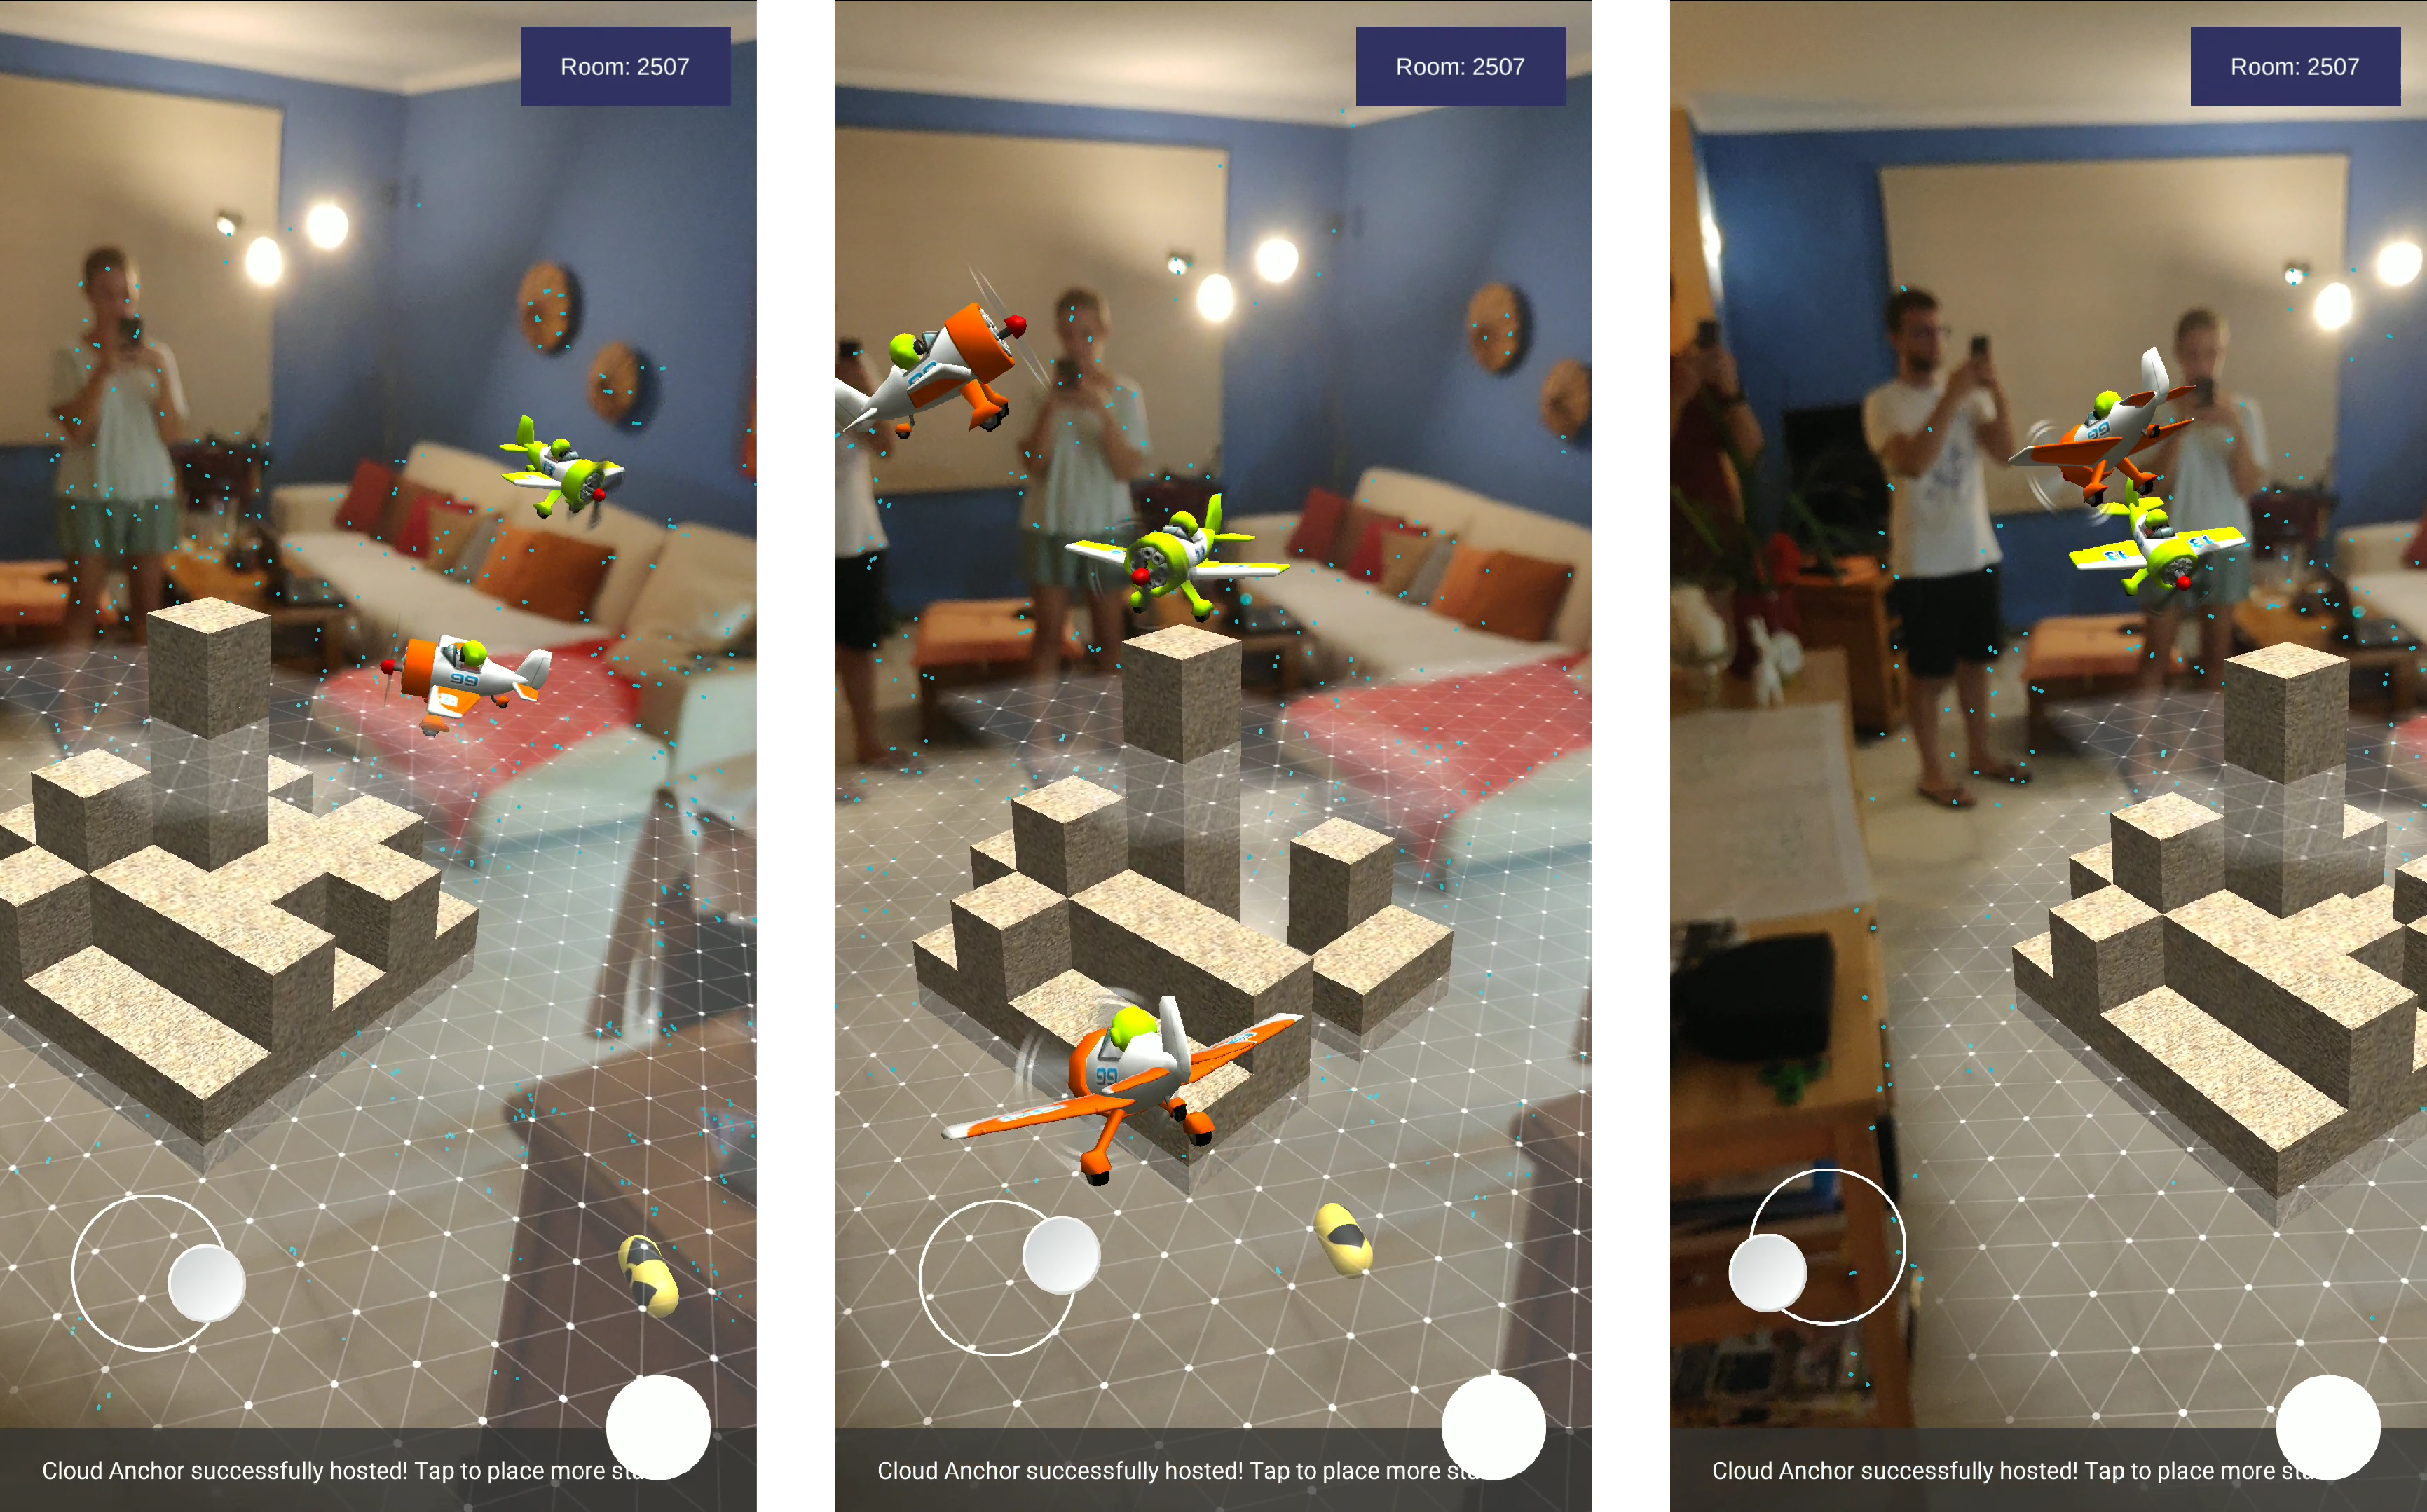
\includegraphics[width=\linewidth]{Images/bombardero.png}
    \caption{Visualización del BombARdero+}
    \label{Bombardero}
\end{figure}

Los Cloud Anchors suben la información del punto de anclaje a la nube, permitiendo compartir esa información con otro dispositivo. Para usarlos, hace falta conseguir una clave de licencia de \textit{ARCore Cloud Anchor API} en Google Cloud Platform~\cite{GCloud}. Una vez conseguida la credencial, hay que introducirla en Unity3D, ``Edit -> Project Settings -> Google ARCore -> Cloud Anchor API Keys''. En los ejemplos que ofrece Google, la implementación de los Cloud Anchor utiliza la \textit{Multiplayer High Level API(Multiplayer HLAPI)} de Unity, por lo que también hay que activar el servicio de multijugador en nuestro proyecto desde el \textit{dashboard} de Unity~\cite{UnityDashboard}. Una vez realizado estos dos pasos, al compilar la escena de ejemplo, debería funcionar. En esa escena, un usuario tiene que crear una sala e instanciar un objeto, el punto de anclaje principal, que se convertirá en las coordenadas (0,0,0) del entorno.
Este punto de anclaje tarda unos diez segundos en subirse a la nube y estar disponible para más usuarios, que al entrar a la aplicación le aparece un listado con las salas disponibles.\\

 Primero tuvimos que mirar como funciona la implementación de Google de los \textit{cloud anchors}, para entender el proceso de cómo se subía el punto de anclaje a la nube y la cantidad de información de control que teníamos. Este proceso fue bastante sencillo, ya que el código de ejemplo es muy entendible e intuitivo. Una vez conseguido implementar con los \textit{cloud anchors} el BombARdero (que habíamos programado anteriormente en monojugador), hubo que hacer retoques a los \textit{scripts} y añadir componentes de la multiplayer HLAPI a los objetos, para implementar la parte multijugador.\\

En el \textit{Cloud Anchor Network Manager} hay que registrar el objeto que se va a instanciar cada vez que entra un jugador a la partida, en nuestro caso es un avión. El avión en un principio está desactivado y se activa en el momento en el que se almacena o resuelve el ancla principal.\\

\clearpage
\noindent